\chapter{Measurements}
This chapter aims to validate the accuracy of force estimation from sEMG after different processing techniques by comparing it to measured data. The goal is to measure sEMG from biceps and triceps, and record sEMG reference noise, and measure the estimated force using a load cell during an exercise of isometric contraction. The sEMG data is then processed using the different techniques that are discussed in the simulation chapter, and the final estimated force will be compared to the measured force. 

\section{Experimental setup}
The measurement setup consists of the following components:
\begin{itemize}
    \item Siemens Single Point Load Cell, 20kg Range, Compression Measure
    \item Keysight E3631A DC power supply at 2V to power the load cell
    \item TMSi Refa8-16e 16 channel amplifier
    \item Kendall H124SG Foam-Hydrogel ECG Electrodes 
\end{itemize}

The 16 channel amplifier performs unipolar measurements. This means that each electrode is connected to its own amplifier channel, and the measured values are compared to the value of a reference. The opposte of unipolar is bipolar which entails that the potential difference between two electrodes is amplified by a single amplifier channel \cite{tmsi_unipolar_bipolar}. 

The load cell has 4 relevant terminals. Two terminals are connected to the power supply to supply the load cell with power. The other two terminals are connected to the amplifier. The 'common' terminal of the power supply is connected to the 'Patient ground' on the amplifier.

Sets of two electrodes are placed on the subjects right bicep, right tricep, and left arm. The electrodes were placed following SENIAM guidelines \cite{seniam}. Two electrodes per set is chosen to essentially capture more data. Since each electrode in a set measures almost identical sEMG signal the signals from the electordes can be averaged to reduce any present noise. The electrodes on the left arm are used to record a reference noise. It is expected that this reference noise has an identical frequency spectrum as the noise present in the sEMG signal since it is recorded at the same time, approximately same place, using the same amplifier, and can therefore be used in some of the presented filtering techniques. The reference signal is recorded using a TMSi provided armband that was wetted and connected to 'Patient ground' on the amplifier. A total measurement setup diagram is shown in figure \ref{fig:measurement_setup_diagram}.

\begin{figure}[h!t]
	\begin{center}
		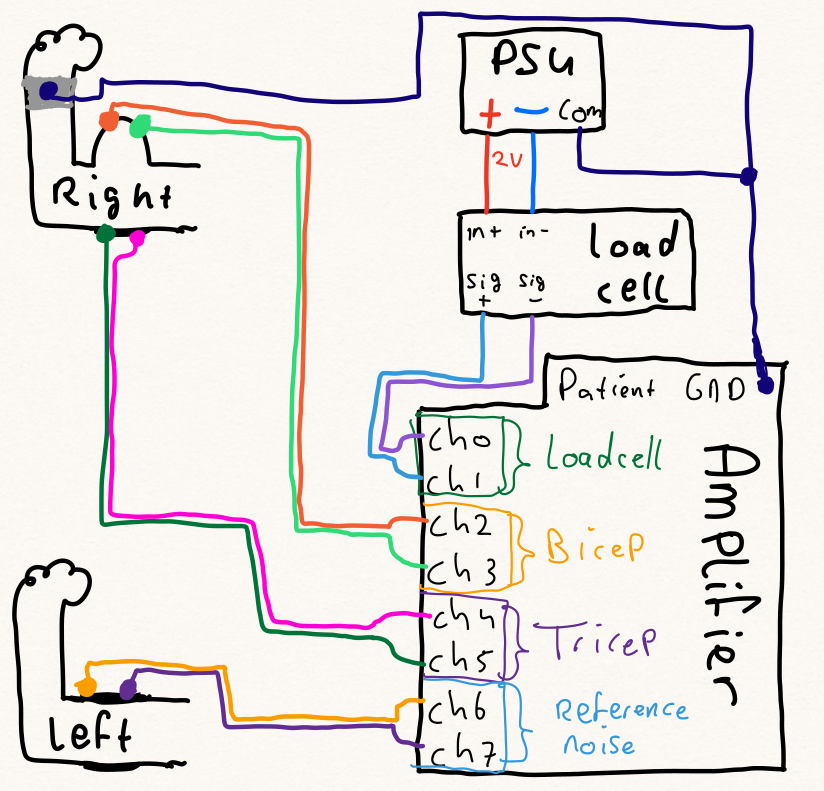
\includegraphics[width=1.0\columnwidth]{images/measurement_setup_diagram.png}
	\end{center}
	\caption{Diagram of the measurement setup}
	\label{fig:measurement_setup_diagram}
\end{figure}

\textcolor{red}{Todo: insert picture of holding load cell handle}

A total of four signal sets were recorded. Two measurements of applying force to the load cell at a sampling rate of \SI{1k}{\hertz} and \SI{20k}{\hertz}, and two accompanying load cell calibration measurements where an object with known weight was attached to the load cell at the sampling frequencies.

The applied force followed the following pattern:
\begin{itemize}
    \item Slowly pulling the handle upwards followed by a slow pushing the handle downwards. Repeated three times
    \item Slowly pull the loadcell upwards followed by returning to a netrual position. Repeated three times
    \item Slowly push the loadcell downwards followed by returning to a netrual position. Repeated three times
    \item Quickly pull the handle upwards followed by a quick push of the handle downwards. Repeated three times
\end{itemize}

\section{Measurement data}

\begin{figure}[h!t]
	\begin{center}
		\includegraphics[width=1.0\columnwidth]{images/measurement_calibration2_1k.png}
	\end{center}
	\caption{Calibration measurements at \SI{1k}{\hertz} sampling rate. The force channels have been lowpassed with a cut-off frequency of 10 Hz to remove large \SI{50}{\hertz} noise component. The offset was determined to be \SI{2.5}{\micro\volt}. The weight op the object was \SI{1681g}{\gram} which corresponds to \SI{167.5}{\micro\volt}}.
	\label{fig:calibration_1k}
\end{figure}

\begin{figure}[h!t]
	\begin{center}
		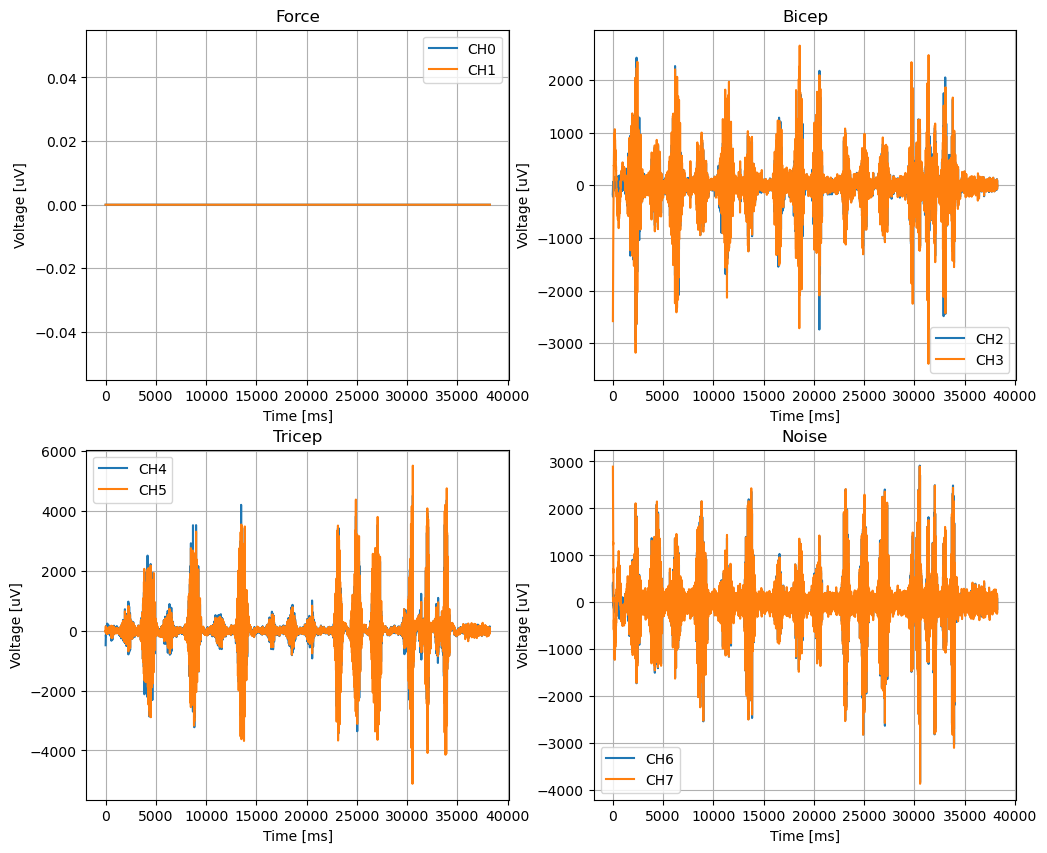
\includegraphics[width=1.0\columnwidth]{images/measurement_meting2_1k.png}
	\end{center}
	\caption{Force measurements at \SI{1k}{\hertz} sampling rate}
	\label{fig:measurement_1k}
\end{figure}

The calibration process required measuring the steady-state value to determine the offset. To relate the measured values to the applied force, an object of known weight was attached to the load cell. These processes can be seen in figure \ref{fig:calibration_1k}. The measured force is approximately 10x the measured signal ($1681g / 167.5 uV = 10.03$).

Due to unknown reasons the amplifier was not able to capture both sEMG signals and the load cell signal at the same time which can be seen in figure \ref{fig:measurement_1k}. The load cell could be measured, but when attaching the the reference armband that the subject was wearing to 'Patient ground' on the amplifier the measured load cell signal was promptly nullified. Attaching the reference armband is required to measure sEMG signals, but connecting this armband makes it impossible to capture load cell information.

\section{Measurement processing result}

Data that was NOT working, data that WAS working, notable characteristics of the data


\section{Conclusion}
Draw numeric conclusion from data, in which situations is which filter how much better?